% !TeX spellcheck = ru_RU
%pdflatex, utf8
\documentclass[unicode, 10pt, a5paper, oneside]{article}

% Установка полей страницы
%\usepackage{anysize}
%\marginsize{0.3cm}{0.3cm}{0.3cm}{0.3cm}
\usepackage[a5paper, margin=0.3cm, bindingoffset=0cm]{geometry}

% Поддержка русского языка
\usepackage[T2A]{fontenc}		% Корректная кодировка шрифта при использовании cm-super
\usepackage[utf8]{inputenc}		% Кодировка ввода
\usepackage[russian]{babel}		% Словарь расстановки переносов
%\usepackage{cmap}				% Перекодировка символов в pdf при использовании обычного cm

% Всякие математические фишки
\usepackage{amsmath}
\usepackage{amsfonts}
\usepackage{amssymb}

% Изменение цвета, работа с графикой
\usepackage{color}
\usepackage[pdftex]{graphicx}
\graphicspath{{images/}}

% Команда для вставки ссылок \url{URL}
\usepackage[hyphens]{url}
\urlstyle{rm}					% Стиль шрифта ссылок: с засечками

% Кликабельные ссылки внутри документа
\usepackage[unicode]{hyperref}

% Включает отступ у первого абзаца в разделе
\usepackage{indentfirst}

% Настрйока стиля списков
\usepackage{enumitem}
\setlist{noitemsep, leftmargin=*, labelindent=\parindent, topsep=0pt, parsep=0pt, partopsep=0pt}

\setlist[itemize,1]{label=$\diamond$}
\setlist[itemize,2]{label=\textendash}
\setlist[itemize,3]{label=$\star$}

\renewcommand{\alph}[1]{\asbuk{#1}} % Костыль для кирилической нумерации вместо латинской
\setlist[enumerate,1]{label=\arabic*)}
\setlist[enumerate,2]{label=\alph*)}
\setlist[enumerate,3]{label=(\arabic*)}


\usepackage{textcomp}			% Команды для вставки разных символов (градусы, проценты, итд)
\usepackage{float}				% Размещение плавающих объектов там где они созданы (X)
\usepackage{wrapfig}			% Обтекаемые текстом рисунки

% Подписи у флоатов
\setlength{\intextsep}{0pt} % Отстут вокруг плавающих окружений
\usepackage{caption}
\captionsetup{parskip=0pt}
\captionsetup[figure]{labelsep=period,justification=centering,singlelinecheck=false,textfont=small,labelfont=small,aboveskip=2pt,belowskip=0pt}

% Изменение формата заголовков разделов
\usepackage{titlesec}
\titleformat{\section}{\newpage\small\bfseries}{\thesection. }{0pt}{}{}
\titlespacing*{\section}{0pt}{0pt}{0pt}

\titleformat{\subsection}{\small\bfseries}{\thesubsection. }{0pt}{}{}
\titlespacing*{\subsection}{0pt}{0pt}{0pt}

\usepackage{array}				% Позволяет объявить свои типы колонок
\usepackage{calc}				% Математика, исп-ся для расчёта ширины колонки
\usepackage{longtable}			% Длинные таблицы

% Минимальный отступ в таблицах
\setlength{\tabcolsep}{1.5mm}

% Новые типы колонок. Ширина задётся как доля от linewidth
\newcolumntype{L}[1]{p{#1\linewidth-2\tabcolsep-2\arrayrulewidth}}
\newcolumntype{C}[1]{>{\centering}p{#1\linewidth-2\tabcolsep-2\arrayrulewidth}}
\newcolumntype{R}[1]{>{\raggedleft}p{#1\linewidth-2\tabcolsep-2\arrayrulewidth}}
\newcolumntype{U}[2]{p{#1\linewidth-(#2)}}

% Стараться не оставлять одиноких строк в начале и конце абзаца
\clubpenalty=1000
\widowpenalty=1000

% Расстановка отступов и переносов
\emergencystretch=2.5em			% Максимальный промежуток между словами
\tolerance=2000
\frenchspacing


\begin{document}

\setcounter{section}{40}

% Вопрос 41 --------------------------------------------------------
\section{Основные этапы автоматизации:  их характеристики и особенности}

\underline{Этапы развития автоматизации}

\textit{Первый этап} --- автоматизация цикла обработки с целью получения заданной формы, размеров и качества обрабатываемой поверхности, цикла сборки для фиксации сборочного соединения.

Средства автоматизации --- ЧПУ обеспечивающие эффективное использование технологического оборудования только в крупносерийном и массовом производстве.

\textit{Второй этап} --- наряду с автоматизацией цикла обработки (сборки) обеспечивается автоматизация загрузки и разгрузки основного технологического оборудования. Такое оборудование оснащено магазинами заготовок и готовых деталей в виде комплектов под сборку и загрузочными устройствами, приспособленными в обслуживанию определенной номенклатуре деталей, функции загрузки-разгрузки может выполнять ПР, установленный совместно с ЧПУ, который обеспечивает возможность использования оборудования в серийном производстве.

\textit{Третий этап} --- предусматривает автоматизацию контроля за ходом выполнения техпроцесса и его оптимизацию. При этом выделяется 2 вида контроля:
\begin{itemize}
	\item проверки соответствия заготовок (комплектующих деталей при сборке), инструмента, состояния технологического оборудования установленным характеристикам с целью внесения коррекции настройкой оборудования или удаления из потока некондиционных деталей.
	\item проверка текущего состояния инструмента и оборудования путем измерения силовых, температурных деформаций и сравнения текущих параметров с эталонными.
\end{itemize}

Таким образом, учитывается влияние случайных и систематических факторов на характер тех. процесса.

\textit{Четвертый этап} --- обеспечивается автоматизация переналадки оборудования на обработку (сборку) объектов производства другого назначения. Это возможно при использовании, к примеру, обрабатывающих и сборочных центров, оснащенными ПР с наборами сменных инструментов, захватных устройств, системы накопителей под номенклатуру обрабатываемых или собираемых узлов (деталей) и оснастки. В этом случае размер изготовляемой партии изделий не имеет значения, ограничивающего гибкость робототехнического производства, классификация (признаки классификации).


% Вопрос 42 --------------------------------------------------------
\section{Назначение, классификация и области применения роботов}

Можно разделить на 3 класса:
\begin{enumerate}
\item	манипуляционные или роботы манипуляторы;
\item	информационные;
\item шагающие
\begin{itemize}

\item  роботы-экзоскелеты (медицинские, роботы-усилители);
\item шагающие аппараты.
\end{itemize}
\end{enumerate}
Манипуляционные: 
\begin{enumerate}
\item	промышленные (универсальные, специальные, специализированные);
\item погрузочные манипуляторы;
\item	для экстремальных сред (космические, подводные, для радиоактивных сред, для токсичных сред, взрывобезопасные);
\item	медицинские;
\item	бытовые;
\end{enumerate}
Наиболее обширен класс роботов-манипуляторов.

Класс информационных роботов включает в себя аппараты для исследования космического пространства,подводного дна и т.п. Они предназначены для автоматического получения и передачи информации об исследуемых объектах.

Класс шагающих роботов включает в себя а), кто предназначены для восстановления двигательных функций человека или для технического усиления мощности двигательных конечностей здорового человека (б).


% Вопрос 43 --------------------------------------------------------
\section{Манипуляционные роботы: типы, характеристики, применение}

Они представляют собой техническую систему, заменяющую труд человека, в состав которого входят орган воздействия на окружающую среду, т.е манипуляционные устройства или манипулятор-это исполнит. Орган, имитирующий действие человеческой руки в достаточно широком диапазоне масштабов увеличения или уменьшения ее геометрических размеров и мощности.

Обобщенная функц. схема манипуляционного робота имеет следующий вид:
\begin{figure}[H]
\centering
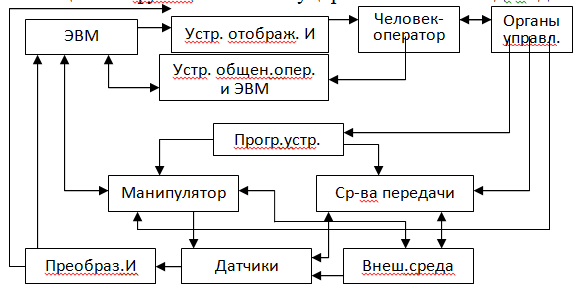
\includegraphics[width=0.8\textwidth]{44_Manipul_robot.png}
\caption{Обобщенная функциональная схема манипуляционного робота}
\end{figure}

Различные группы манипуляц. роботов включают в себя ту или иную часть блоков и связей, составляющих обобщенную схему.

Манипуляц. робот м. иметь 1 или несколько манипуляторов. Движения манип-ров м. отличаться от движения руки ч/а. В суставах, звеньях манип-ров м. не только вращаться, но и перемещаться поступательно. М. изменяться длина некоторых звеньев. Кисть руки имитируется с пом. захвата (м.б. 2-хполый, 3-хпалый или более). На захвате м.б. установлены различные датчики.

Средства передвижения м.б. колесными, гусеничными, шагающими, плавающими и т.д.
Устанавливаемые датчики И. позволяют роботу ориентироваться во внешней среде.
По способу упр-я манипуляц. роботов разделяют на 3 группы: автоматич.,биотехнические, комбинированным управлением.

\textit{Автоматическими} манипуляц. роботами называют  устройства, ктр. действуют без непосредственного участия ч/а в упр-ии. Они прим-ся в тех случаях, когда манипуляц. устр-во удалено на значит. расст. от органов упр-я, либо когда очень высокий темп работ, опасны внешняя среда или объект действия, а ручное упр-е нецелесообразно.
Выделяют: I покол.(программн, интеллектуальные, адаптивные).

\textit{Биотехнич.} манипуляц. роботы --- робот, в систему упр-я ктр-х включен человек-оператор. М.б.: командные --- упр-ся оператором дистанционно с командного устр-ва с нажатием кнопок или с помощью упр-щей рукоятки.

\textit{Копирующие} манипуляц. роботы имеют задающий орган, геометрически подобный манипуляц-ому устр-ву. При этом способе упр-я привод каждого звена вместе с соответствующим датчиком образует дистанционно следящую систему. Если положения задающего органа и манипуляц. устр-ва совпадают, то последнее стремится к 0 ошибке по положению.


% Вопрос 44 --------------------------------------------------------
\section{Структура механизмов манипуляционных роботов и характеристики их геометрических свойств}

Механизмом называют механич. систему, предназначенную для получения требуемого движения 1-го или нескольких тел.

Основными элементами являются: звенья и кинематич. пары.

Звено-1 или неск жестко соединенных твердых тел, входящих в состав механизмов.
Звенья:
\begin{enumerate}
\item простые состоят из 1-го твердого тела;
\item составные --- из нескольких твердых дел.
\end{enumerate}

Кинематич. пара --- соединение двух смежных звеньев, допусккающие их относит. движение. Звенья м. соприкасаться пов-тями, линиями и точками.

Кинематич. пара м.б. плоской, если относит. движение сочлененных звеньев возможно лишь в параллельных плоскостях или в пространстве, если относительное движение сочлененных звеньев возможно в любом направлении.

С целью уменьшения потерь и увеличения износостойкости между звеньями вводят промежуточные элементы (ролики или шарикоподшипники). Такие совокупности образуют кинематич. соединение.

Кинематич. пары классифицируются по числу условий связи на относительное движение двух смежных тел или по числу степеней свободы. Каждое условие связи кинематич. пары не только устраняет относительную подвижность, но и позволяет передавать от звеньев к звеньям силовое воздействие.

Свободное тело в пространстве имеет 6 степеней своб:3 поступательные движения в направлении оси x,y,z, 3 вращательных движения относительно этих осей.

Если 1 звено превратить в стойку, то для 2-го звена в соответствии с конструкцией кинематич. пары: W=G-U, U-число связей, налагаемых кинематич. парой на относительно движения ее звеньев. При U=0 пара отсутствует, т.к. отсутствуют связи между звеньями. При U=6 относительного движения звеньев нет, т.к. они образуют 1 звено. Поэтому число условий связи кинематич. пар м. находиться в пределах от 1 до 5. Соответственно этому все кинематич. пары делят на 5 классов или на 5 родов по числу степеней свободы.

Кинематич. пары 1 и 2 классов в манипуляц-х роботах не применяются. Примеры кинематич. пар манипуляц. устр-в:
Класс 3, род 3 --- 3 степени свободы, класс 4, род 2 --- 2 степени свободы.

Кинематич. пара 3 класса 3 рода предст. собой шаровой шарнир , имеющий 3 степени свободы-вращение относительно каждой из осей.

Кинем. пара 4 класса 2 рода м.б. реализована либо вращением одной из осей, указанных в системе коорд. и поступат. движ. Вдоль 1 оси, либо вращение относит. двух взаимоперпендикулярных осей.

Кин. пара 5 класса 1 рода позволяет иметь лишь одно относит. движение-либо вращение, либо поступат. движение вдоль 1 оси.

Кинемат. цепью называют связанную систему звеньев, образующих кинематич. пару. Они бывают замкнутыми и открытыми. Замкнутая кинемат.цепь --- такая цепь, в ктр.звенья входят не менее, чем в 2 кинемат. пары. Открытая кинем. цепь --- цепь, в ктр. имеются отдельные звенья, входящие только в 1 кинем. пару.

Механизм манипуляц. робота представляет собой сложную открытую кинем. цепь, у ктр-х 1 звено обращено в стойку, а движение вых-х звеньев вполне опр-ся заданным движением входных звеньев.

Манипуляц. устр-ва предст. собой открытую кинематич. цепь, в ктр. число n подвижных звеньев всегда = числу кинематич. пар. Тогда число степеней свободы для механизма манипуляц-го устр-ва опр-ся как: \begin{equation}
W=3p3+2p4+p5
\end{equation}
\begin{equation}
n=p3+p4+p5
\end{equation}

Пространств. исполнит. механизмы м. иметь большое число степеней свободы во многих отношениях они аналогичны руке человека. Однако число звеньев чел. руки достаточно велико (n=19) и число степеней свободы W=27. В наст. время ни один механизм не обладает такими возм-тями . Однако при существующем уровне техники-это не так уже важно.

Характеристики геом-х св-в манип-х устр-в:
\begin{enumerate}
\item  \underline{Зона обслуживания}

У манипуляц-х устр-в выделяют базовую плоскость, плоскость ктр образована плечом и предплечием мнипулятора и в ктр м. располагаться одновременно оси всех его звеньев.

Зоной обслуживания манипуляц-го робота называют сов-ть точек базовой плоскости, ктр. м. достигать захват манипуляц-го устр-ва. Преимущественное распространение получили манипуляторы с упорядоч-м расположением звеньев кинематич-х пар , т.е. такие, когда имеется 1 пара смежных кинематически связанных звеньев, ктр обеспечивает перенос кисти в базовой плоскости в любую точку зоны обслуживания.

\item \underline{Рабочий объем} или рабочие зоны манипуляц-го устр-ва называют пространство , ограниченное поверхностью, огибающей все возможные положения захвата. Для обеспечения наиболее полного обслуживания любой точки необходим механизм манип-ра, исп-щий не менее 6 степеней свободы, из ктр-х 3-для перемещения кисти, 3-для ориентации захвата кисти. Тогда в зависимости от сочетания кинем. пар, обеспечивающих перемещения кисти различают 3 осн.формы рабочего объема:
\begin{itemize}
\item	прямоугольный, когда кисть пеермещается в пространстве с пом. Механизма с 3-мя поступат-ми кинем-ми парами 5 класса;
\item цилиндрич., когда исп-ся механизм с двумя поступательными и 1 вращательной кинем.парой;
\item сферический, когда исп-ся 2 вращат. и 1 поступат., либо 3 вращат. кинематич. пары.
\end{itemize}
\item  \underline{Движение манипуляц. робота} и его манипуляц-го устр-ва. Для манипуляц-х роботов вводят понятие глобальных, региональных и локальных движений.

К глобальным движениям робота относят его перемещ-я в пространстве с пом. средств передвижения.
Регион.движения робота-это движения по переносу кисти его манипуляц-го устр-ва в любую точку рабочего объема.

Локальные движения робота связаны с ориентацией кисти в пространстве и движение по захвату объектов действий, движение манипулятора в его рабочем объеме м. классифицировать:
\begin{itemize}
\item	Движение манипуляц-го устр-ва, несущего своб. объект и совершаемые в своб. объеме
\item	Целенаправленное движение манипуляц-го устр-ва по перемещению своб-го объекта, совершаемые в несвободном рабочем объеме
\item	Движение манипуляц-го устр-ва в своб. объеме, согласованные с движением объекта действия
\item	Движения манипуляц-х устр-в в несвоб.объеме, согласованные с перемещением объекта действий.
\end{itemize}
\item \underline{Маневренность}

Ключевой А и запястный кистевой механизм С имеют каждый 3 степени  свободы. Они позволяют ориентировать кисть 3 на нектр. Участки поверхности сферы с радиусом, равным пределе сумм длин плеча 1 и 2.
Кинематич.пара 5 класса в локтевом суставе В позволяет менять радиус сферы и доставлять захват в любую точку сферического рабочего объема.
Если зафиксировать захват 4 неподвижные точки. Манип. устр-во будет иметь возможность совершать круговое движение плечами 1 и 2. Т.о. св-ва манип-го устр-ва м. иметь подвижность при фиксированном захвате называется маневренностью. В рассм-вом случае механизм сохраняет 1 степень свободы, что оперделяет степень маневренности манип. устр-ва.

Повышение числа степеней маневренности позволяет выполнять движения более сложных классов, сужает мертвые зоны манип-го устр-ва и увеличивает свободу действий оператора.

Перестановка кинем. пар в данном устр-ве, н-р, А вместо В не меняет число степеней свободы, но при фиксированном захвате превращение манипуляц. устр-во в ферму и механиизм теряет свою маневренность.
\end{enumerate}


% Вопрос 45 --------------------------------------------------------
\section{Приводы манипуляторов и роботов: классификация, особенности применения}

В зависимости от используемого вида энергии приводы подразделяют на гидравлические, пневматические, электрические и комбинированные (например, электрогидравлические, гидропневматические и др.) Часто их применяют в комбинации, например, в звеньях манипулятора большой грузоподъемности используют гидравлический привод, а в его захватном устройстве --- более простой и маломощный пневматический.

\underline{Пневматические} приводы применяются в 20…30\% (по другим оценкам в 40-50\%) серийно выпускаемых ПР. Их используют  для легких и средних (по грузоподъемности до 20 кг) ПР при числе степеней подвижности 2…3. Погрешность позиционирования в этих приводах не превышает ± 0,1 мм. Скорость ведомого звена привода при линейном перемещении составляет до 1000 мм/с, при угловом --- до 60 об/мин. Они имеют простую конструкцию, низкую стоимость и достаточно надежны в работе.

Вследствие низкой регулировочной способности их мало используют в позиционных и контурных режимах работы, и они имеют цикловое управление, как простейший вариант позиционного (задается две точки --- начало и конец перемещения).

\underline{Гидравлические} приводы применяются в 30\% серийно выпускаемых средних и тяжелых ПР при числе степеней подвижности 3…4. Погрешность позиционирования в этих приводах не превышает ± 0,5 мм при скорости линейного перемещения до 0,8…1200 мм/с. Эти приводы имеют сложную конструкцию, высокую стоимость изготовления и эксплуатации. Гидравлический привод имеет хорошую регулировочную способность, и его используют в ПР с позиционным и контурным режимом работы.

\underline{Электрические} приводы используются в 40…50\% серийно выпускаемых ПР со средней грузоподъемностью и числом степеней подвижности 3…6. Точность позиционирования электрического привода достигает значений до ± 0,05 мм. Их применяют как в позиционном, так и в контурном режимах работы. 

Преимуществами электроприводов являются более высокая экономичность, КПД, удобство сборки и хорошие регулировочные свойства. 

Как правило, в электроприводах используют синхронные, шаговые и двигатели постоянного тока. Асинхронные двигатели применяются реже, что связано с трудоемкостью управления частотой вращения.

\underline{Комбинированные} приводы позволяют максимально использовать достоинства отдельных типов приводов. Чаще всего в промышленных роботах применяют комбинацию пневматического и гидравлического приводов (пневмогидравлические и гидропневматические), а также электрического и гидравлического (электрогидравлические). В конструкциях ПР пневмогидравлические приводы имеют ограниченное применение. В них в качестве исполнительного органа используется пневмоцилиндр, а стабилизация его скорости и гидравлическая фиксация осуществляется гидросистемой.

В гидропневматическом приводе в качестве исполнительных двигателей применяют гидродвигатели, а пневмосистема применяется для создания необходимого давления в гидросистеме, что позволяет отказаться от гидронасосных станций.

% Вопрос 46 --------------------------------------------------------
\section{Конструкции схватов промышленных роботов, особенности применения}

Промышленный робот (ПР) --- это универсальное, автономное и автоматическое устройство с памятью и программным управлением, предназначенное для воспроизведения двигательных и некоторых умственных функций человека при выполнении основных и вспомогательных производственных операциях.
Основной частью ПР являются манипуляторы.

Под конструкцией роботов понимается конструктивное исполнение их механической системы.
В общем виде их механическая система состоит из следующих элементов:
\begin{itemize}
\item опоры, в виде основания или передвижных тележек напольного или подвесного типа;
\item корпуса робота различной формы с вмонтированными в него механизмами подъема и поворота руки и перемещения робота;
\item корпус руки робота с вмонтированными в него механизмами перемещения руки, звена, а в некоторых случаях, и захвата руки;
\item руки робота с одним или несколькими звеньями;
\item захватного устройства.
\end{itemize}

Захватные устройства служат для захватывания, базирования и удержания объекта в определенном положении. Эти объекты могут иметь различные материалы, форму, объем, массу. Обычно, в зависимости от этих показателей робот в пределах своей области применения имеет определенный набор ЗУ.
При необходимости робот оснащают специальными ЗУ в виде присосок, губок и другие для захвата специальных объектов. При этом, для надежности захвата применяют такое усилие, которое необходимо для удержания объекта, но не оставляло бы следов губок на его поверхности и не изменяла бы форму объекта.

Классификация ЗУ:
\begin{enumerate}
\item	По способу удержания объекта:
\begin{itemize}
\item	схватывающие
\item	поддерживающие
\item	удерживающие
\end{itemize}
\item	По принципу действия:
\begin{itemize}
\item 	механические
\item	с эластичными губками или камерами
\item	вакуумные
\item	магнитные
\end{itemize}
\item	По характеру базирования объекта:
\begin{itemize}
\item	центрирующее
\item	базирующее
\item	фиксирующее
\item	способное к перебазированию
\end{itemize}
\item	По степени специализации ЗУ:
\begin{itemize}
\item	универсальные (с широким диапазоном захвата)
\item	многоцелевые ( приспособленные для захвата по определенной номенклатуре поверхностей)
\item	целевые (предназначены для захвата только определенной группы деталей)
\item	специальные ( для определенного объекта)
\end{itemize}
\item	По рабочему диапазону:
\begin{itemize}
\item	широкодиапазонные для захвата различных поверхностей
\item	узкодиапазонные
\end{itemize}
\item	По наличию дополнительных устройств и механизмов:
\begin{itemize}
\item	без устройств
\item	с устройствами для ориетационных перемещений
\item	с приспособлением для выполнения технологических операций
\end{itemize}
\item	По числу рабочих позиций:
\begin{itemize}
\item	однопозиционный
\item	многопозиционный
\end{itemize}
\item	По характеру работ ЗУ:
\begin{itemize}
\item	последовательно
\item	параллельно
\item	комбинированный
\end{itemize}
\item	По виду управления ЗУ:
\begin{itemize}
\item	неуправляемый
\item	командный
\item	адаптивный
\item	жесткопрограммный
\end{itemize}
\item	По характеру крепления руки робота:
\begin{itemize}
\item	не сменяемые
\item	сменные
\item	быстросменные
\item	пригодные для автоматической смены.
\end{itemize}
\end{enumerate}

К ЗУ предъявляются требования общего характера и специальные, связанные с конкретными условиями эксплуатации.

К числу обязательных:
\begin{itemize}
\item	надежность захватывания и удержания объекта;
\item	стабильность базирования;
\item	недопустимость разрешения объекта.
\end{itemize}

Прочность ЗУ должна быть высокой при малых габаритных размерах. Особое внимание должно быть обращено на надежность крепления ЗУ к руке ПР.

К ЗУ работающих в условиях серийного производства существуют дополнительные требования:
\begin{itemize}
\item	возможность захватывания и базирования деталей в широком диапазоне массы, размеров и формы;
\item	обеспечение захватывания близко расположенных деталей;
\item	легкость и быстрота замены ЗУ.
\end{itemize}

В ряде случаев необходимо автоматическое изменение усилия удержания деталей.
ЗУ является основным рабочим органом робота, имеет очень разнообразные схваты, поэтому разработана стандартная таблица основных типов объектов, т.е. деталей:
\begin{enumerate}
\item Для деталей типа тел вращения:
\begin{itemize}
\item центрирующие
\item	базирующие
\item	с эластичным покрытием
\item	вакуумные.
\end{itemize}

Причем, здесь различаются ЗУ двух типов: для деталей типа втулок и типа валов, причем в последнем случае применяются только центрирующие ЗУ или захватные по наружному зазору.
\item Для плоских деталей, применяются, в основном, базирующие.
\item Для деталей коробчатой формы, те же, что и в первом случае (того же типа), кроме центрирующих.
\item Для нессиметричных деталей, те же, кроме центрирующих и эластичных, В основном, эти детали обрабатываются со спутниками и в зависимости от формы спутника.
\end{enumerate}

% Вопрос 47 --------------------------------------------------------
\section{Проектирование  архитектуры интегрированной компьютерной системы управления }

Целью ИКСУ является обеспечение условий для взаимосвязанного согласованного управления конструкторско-технологической подготовки произ-ва и упр-я производственными и технол-ми процессами. Методология проектирования таких систем ---разделение объекта автоматизации на части, позволяющей осущ-ть эффективную автоматизацию ккаждой из них.


Применительно к иерархически организованных СУ различают горизонт. и вертик. интеграцию. В общем случае, горизонт. интеграция предполагает объединение АС 1-го уровня.Н-р, АС проектных работ производственного процесса.

Вертикальное-объединение разных уровней, в частности, вертик. Интеграция предполагает объединение САПР, автоматизации тех. процесса, а также корпоративных систем(экон-х, финансовых упр-ий персоналом) в единую интегрированную инф. Сеть, что обеспечивает обмен данными между всеми подразделениями упр-ческого уровня.

В наст. время вертик. интеграция формируется путем организации потоков И. от нижнего уровня (датчики, контроллеры АСУТП), от КД САПР во внутр. выч. сети участков и цехов(MES) и далее выч.сети предпр. в целом(ERP).

Сущность технологии открытых систем состоит в формировании среды, вкл-щей ПО, аппар.ср-ва, службы связи интерфейса, форматы данных и протоколы, обеспечивающие переносимость, масштабируемость и взаимосвязь приложений и данных. Сов-ть этих качеств достигается исп-ем общепризнанных стандартов на ИТ. Основным приемом построения служит национ.стандартизация или построение профиля.

Профиль-согласов. набор базовых стандартов, предназначенные для решения какой-либо задачи или класса задач.

В основе современных архитектур лежат 2 группы моделей: 
\begin{enumerate}
\item модель объектов данных с описанием И.,циркулирующей в ИКСУ;

\item операц.модели, опр-щие процессы преобраз.И.
\end{enumerate}
Для любых из таких моделей выделяют 4 общие группы стандартов:
\begin{enumerate}
\item стандарт на уровни;
\item стандарт на инф.потоки;
\item стандарт на интерфейсы; 
\item стандарт на операции и функции
\end{enumerate}

\textit{S-88, MES, S-95, OPC,ODBC, SQL, CALS, PLM}.

S-88 этот стандарт направлен на увелич.гибкости и прозрачности оборудования  и ПО. Он обслуживает batch-процессы и устанавливает рекомендации по реш.задач, связанных с упр-ем обор-я, безоп-тью, произв.рисками  и контролем производственных операций. Batch-процесс опр-ся как процесс выпуска конечного кол-ва продукции на основе обработки конечного кол-ва входных материалов в соответствии с указанной рецептурой на одной или более единицах оборудования, т.е. в отличие от непрерывного производства эти процессы основаны на использовании ограниченного кол-ва материала. Такие процессы характерны для гибких производственных систем.

В соответствии с требов-ми стандарта ISA S88.01-1995 при проектировании ИКСУ д.б. разработана модель состояний гибкой произв. системы и ТП в целом. Поведение оборудования планируется в виде диагарммы состояний. Т.о., в любой момент времени оборудование м. находиться в 1-м из предполагаемых состояний-остановка, сброс, пуск, работа, подготовка, авария и др.При исп-ии рекомендации данного стандарта контроллер будет исп-ть виртуальную машину состояний для опр-я состояния оборудования в любой момент времени.

ISA S-95 отвечает за решение задач операц-го менеджмента ср-вами инф-х систем. Он опр-ет интерфейсы между бизнес-функциями и произв-ми операциями и служит для интеграции соврем-х систем упр-я. Стандарт описывает модель производственных операций, получившую развитие в системах для исполнения произв. деятельности и содержит примеры док-та отчетности аналитических зависимостей, исп-мых для оценки эфф-ти произ-ва.
%Вставить картинку про 4 уровня.
\begin{figure}[H]
\centering
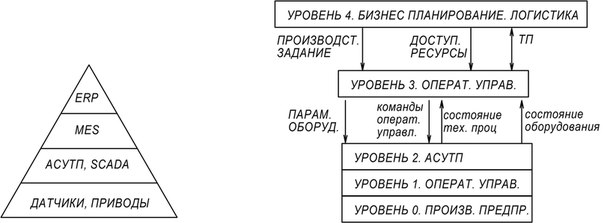
\includegraphics[width=0.8\textwidth]{47_Urovni.jpg}
\caption{Иерархическая модель упр-я согласно ISA-95}
\end{figure}

В 1 части ISA95.00.01 рассм-ся многоуровневая модель обмена И. и связи между ур.4 и 3 (производств.подразделения). 2 часть станд.определяет форматы обмена данными через эти связи в соответствии со схемой взаимодействия . Здесь определены форматы документов для обмена И.по оборудованиям, материалам, персоналам, технологии изготовления, эффективности ТП. 3 часть стандарта ISA95 описывает модели и действия, хар-ные для упр-я произв-вом(ур.3), ктр. обычно поддерживаются след-щими системами: исполнение произв. деят-ти (MES). контроля качества (LIMS) и автоматизированного упр-я активами предприятия (EAM).

Модель произв-ва приводится в действие плановым производством , по ктр-м составл-ся детальные графики, содержащие рабочие задания, действия и события.

Модели деят-ти при упр-ии произ-ми процессами рассмотрены в 4 части стандарта. 5 раздел стандарта посвящен обмену между бизнес-приложениями и производством. В упр-ии произв-ми процессами входят функции упр-я персоналом, обор-ем и материалами. Имеются функции для упр-я рецептурой и технологией произв-ва.

MES-исполнит.система произв-ва.Эти системы решают задачи синхронизации, координируют, анализируют и оптимизируют выпуск продукции.

OPC-стандарт подключаемости компонентов в компь.СУ. Они разработаны с целью сокращения затрат на создание и сопровождение приложений промышленной автоматизации. Их применение решает вопрос обмена данными с устр-вами разных производителей ИМС разными протоколами обмена данными. OPC-это программная технология на базе W-s технологии, представляющей единый интерфейс для упр-я объектами автоматизации. OPC DA описывает набор функций обмена данными в реальном времени с прогр.логическими контроллерами, ЧПУ и др. OPC AE- функции уведомления по требованию о различных событиях(ававрийные ситуации).

Применение OPC предоставляет разработчикам универс.фиксированный интерфейс обмена данными с любыми устр-вами. Разработчики устр-в ввода-вывода дополняют их спец.программой, реализующей интрефейс.

\textit{Достоинства OPC}:

Если заменяется какой-л компонент СУ, то нет нужды корректировать др.ПО, т.к.при замене драйвера поверх нее б.функционировать инсталлирование OPC. При включении нового компонента необходимо правильно сконфигурировать его на программном уровне. Если в систему добавить новую программу, необходима только конфигурация OPC-клиента.

CALS-архит.поддержка сбора данных в течении жизненного цикла продукции. Она обеспечивает единообразные способы упр-я процессами и взаимодействия всех участников этого цикла:заказчиков продукции, поставщиков и производителей экспл-ции и ремонтного персонала.

На предприятии с CAL-технологией реализуется в соответствии с требованиями системы международного стандарта, регламентирующих правила указанного вз-я преимущественно посредством электронного обмена данными.

Применение CALS-технологии позволяет существенно сократить объем проектных работ, т.к. описание составных частей оборудования, машин и систем, проектировавшихся ранее хранится в унифицированных форматах данных, доступных любому пользователю технологии CALS. Главная задачарешения-обеспечения единообразного описания и интерации результатов независимо от места и времени их получения в общей системе. При этом структура проектной технологич. и экспл. док-ции, языки ее представления д.б.стандартизованы, тогда становится реализумой успешная работа над общим проектов разных коллективов, разделенных во времени и в пространстве и использующих разные системы. 1 и та же КД м.б.использована в разных продуктах, а технологическая документация адаптирована к разным производственным условиям.

Для обеспечения инф.интеграции в качестве форматов данных используют стандарты ГОСТ ИСО 10303. В CALS входят также стандарты электронного обмена данными, электронные ТД и руководства для совершенствования процесса.

ODBC-это программный интерфейс доступа к БД, он позволяет единообразно оперировать с разными источниками данных, не учитывая особенности взаимодействия в каждом конкретном случае.Это достигается благодаря тому, что поставщики различных БД создают драйверы, реализующие конкретные дополнения функций ODBC с учетом особенностей их продукта.

SQL-язык структурированных запросов, универс.компь.язык для создания, модификации и упр-я данными в реляционных БД.Это язык манипулиров-я данными , ктр. позволяет описывать условия поиска И., не задавая для этого последовательность действий.

PROFINET предназначендля коммуникационной части систем промышленной автоматизации.Он обеспечивает доступ к устр-вам полевого уровня (датчики) со всех уровней упр-я предприятием. Стандарт позволяет выполнять широкий обмен данными и использует стандарты вплоть до полевого уровня: практически все стандарты Ethernet, промышленный протокол CAL.Все они м.б. интегрированы в профильную единую сеть без модификации установленной аппаратуры.

PROFINET использует стандарт TCP/IP для выполнения операций настройки параметров, конфигурирования и диагностики.Обмен данными в реальном масштабе времени выполняется через стандартные каналы связи Ethernet параллельно со стандартными вариантами обмена данными

% Вопрос 48 --------------------------------------------------------
\section{Описание технологического процесса как объекта автоматизированного управления }

Любое производство состоит из множества технологических операций, каждая из ктр-х служит для решения общей задачи выпуска продукции. Даже если большинство технологических операций упр-ся АС(РТК,АСУТП), то это оказывается недостаточной для решения задач упр-я производством, т.к. эти автоматизированные участки обладают собственной логикой работы и оперируют собственным набором данных.

\begin{figure}[H]
\centering
\includegraphics[width=0.6\textwidth]{48.jpg}
\caption{Технологический процесс}
\end{figure}

На рис. показаны типовые каналы упр-я и наблюдения за ТП. Фактически каналы упр-я и наблюдения в реальных технологических модулях, представляющих собой их различную комбинацию.

По функциональному назначению в СУ м. выделить 5 каналов упр-я,ктр. осуществляют разные по характеру воздействия на технологическую систему. 
Канал С1 связан с осуществлением разнообразных дискретных операций (вкл.,выкл. приводов). Число подобных операций м. достигать нескольких сотен и упр-я осущ-ся от спец-го машинного контроллера.

Канал С2 осущ-ет упр-е движ-ми рабочих органов. В зависимости от геометрии изделия на этом уровне м. осущ-ся линейные и круговые перемещения рабочих органов.
С3 отвечает за авоматич. коррекцию формообразующих движений. На этом уровне по результатам измерения обработанных деталей вводятся дополнит. корректирующие возд-вия с целью обеспечения заданной точности.

Каналы С4 и С5 применяются с целью обеспеч-я качества обработки.

Канал С4 связан с активным контролем деталей в процессе обработки, по результатам измерения, отклонений размеров деталей в следствии износа инструментов или деформации осущ-ся под наладкой.

Канал С5 соответствует уровню адаптирования упр-я, осущ-го по результатам измерения силы моментов, деформации с целью изменения параметров процесса обработки.
Для формирования упр-я м. использоваться спец.каналы наблюдения. Различают след.уровни наблюдения:

01 соответствует обнаружению событий об исполнении той или иной команды (осведомит.сигналы, поступающие в систему упр-я для выполнения след.команды).

02-уровень измерения линейных и круговых перемещений. Измерение перемещения и их производных осуществляется измерительными преобразователями различной физической природы.

03-диагностика состояния оборудования, т.е. формирование упр-щих возд-вий м.участвовать и дополнит.измерит.И.,н-р, о параметрах деталей до и после обработки, от состоянии самого технологического модуля, его узлов и т.д.

04-06 контролирование состояний материального потока на входе ТП,н-р,геом. параметры заготовки и инструменты.
Ур.07 и 08 контролируют состояние энергетического процесса. Число уравнений наблюдения м.б.значительно больше уравнения упр-я. Чем более ответственный и качественный ТП, тем больше уровней наблюдения требуется для упр-я технологическим процессом.

% Вопрос 49 --------------------------------------------------------
\section{Описание производственного процесса как объекта автоматизированного управления: реализация АРМ различных уровней}

Описание ПП в целом м.б.представлено в виде карты основных бизне-процессов, на каждый из ктр-х составляется спецификация. Функциональная модель бизнес-процессов представляет собой многоуровневую систему взаимосвязанных диаграмм, содержащую полное описание процессов жизненного цикла произв-ва продукции.

При этом вход I представляет собой то, что перерабатывается процессом, выход О-результат переработки, упр-е С-И., необходимая для выполнения процессов и механизм М ---обеспечение выполнения процессов с использованием его оборудования(построение функциональных моделей регламентируется Р50.1.028-01).Стандартами MES и S95 установлены 8 базовых бизне-процессов

\begin{figure}[H]
\centering
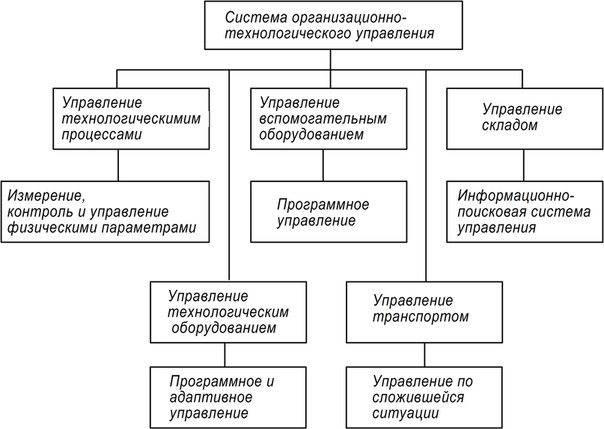
\includegraphics[width=0.6\textwidth]{49_proizv_proces.jpg}
\caption{Производственный процесс}
\end{figure}

Из перечня задач, котор.д.решаться в рамках выполнения этих базовых бизнес-процессов м.б.выделены те, кoтoр.д.б.решены системой интегрированного компь-го упр-я с использованием АРМ различного назначения.

АРМ SCADA-мастера в общем случае д.решать следующие задачи:
\begin{enumerate}
\item диагностирование состояний технологического оборудования;
\item упр-е оборудованием посредством экранных форм (в режимах пуска, останова работы и т.п.);
\item подключение и визуализация заявок на производство продукции;
\item контроль над процессом автоматического изготовления;
\item архивирование технологических и расчетных параметров;
\item представление оперативной И.о выполнении сменных заданий;
\item подготовка отчетов о фактическом использовании оборудования.
\end{enumerate}
АРМ SCADA в диспетчеризации производства:
\begin{enumerate}
\item	отслеживание выполнения операции технол. требований;
\item	отслеживание выполнения заказов, объема и партий;
\item	контроль в реальном времени выполнения работ в соответствии с планом;
\item	анализ производительности;
\item	формирование отчетной документации;
\item	контроль состояния и распределения ресурсов;
\item	отслеживание занятости оборудования.
\end{enumerate}
АРМ SCADA технолога д.вып-ть след.функции:
\begin{enumerate}
\item управление качеством продукции:представление данных измерений о качестве продукции, собранных с технологических линий;
\item мониторинг И.о ходе ТП;
\item отслеживание предупредительной и аварийной сигнализации;
\item оповещение оператора об аварийных и внештатных событиях;
\item представление действий об исправлении ситуаций на основе зависимости и статистических данных;
\item контроль состояния и распределения ресурсов:отслеживание занятости оборудования и коррекция настроечных параметров и задач, сбор и хранение данных, отслеживание историй продукта (где и в каком порядке велась работа с данной продукцией)
\end{enumerate}
АРМ диспетчера по обслуживанию оборудования:
\begin{enumerate}
\item	отображение состояния технологического оборудования и всего комплекса аппаратных средств;
\item	отображение графика ремонтов, формирование заданий и контроль выполнения ремонтных работ;
\item	отслеживание аварийной ситуации в ТП;
\item	отслеживание наработки оборудования.
\end{enumerate}
АРМ менеджера или руководителя:
\begin{enumerate}
\item отслеживание графика изготовления продукции по каждому контракту;
\item	контроль номенклатуры и объемов полуфабрикатной продукции в незавершенном производстве;
\item	контроль планирования и отслеживания выполнения планов по производству
\item	отслеживание решений оперативного планирования.
\end{enumerate}


% Вопрос 50 --------------------------------------------------------
\section{Выбор датчиков технологического процесса: типы измерительных устройств,  подключение.}

При их выборе в ПЗ необходимо провести следующие расчеты исследования:
\begin{enumerate}
\item тип датчика,
\item точность или погрешность измерения,
\item диапазон измерения,
\item единицы измерений,
\item диапазон выходного сигнала датчика,
\item условие эксплуатации(защищенность ВГП,различные требов.к источникам питания, помехозащищенность и т.д.), 
\item интерфейсы связи с компь.средой,
\item стоимость(в т.ч.затраты на экспл-цию).
\end{enumerate}
Интерфейсы выходных сигналов измерительных приборов:
\begin{enumerate}
 \item по типу вых.сигнала:
 \begin{itemize}
 \item аналоговые(электросигнал,емкость,частота,ток: 0-20мА, 4-20мА, 0-5мА; напряжение, сопротивление),
 \item цифровые(двоично-десятичный код, RS232,RS485,HART-протокол,промышленные сети);
 \end{itemize}
\item вторичные измерительные преобразователи(измерит.мосты, самописцы, программируемые логич.контроллеры и др.)
\end{enumerate}
Первичный измерит.преобразователь (ПИП) с токовым аналоговым выходом имеет встроенный источник тока с некоторым внутренним сопротивлением.Источник тока упр-ся функцией f(x) измерения параметров ч:

Ток поступает в линию связи и на входном нагрузочном резисторе ВИП создает соот ветствующее падение напряжения,ктр.далее преобразуется в цифровое значение измеряемого параметра ч. ИП данного вида имеют унифицированные вых.сигналы постоянного тока в различных диапазонах (0-20мА,4-20мА,0-5мА). При этом минимальному значению тока соответствует миним.значение измеряемого параметра. Чаще всего при токовом сигнале 4-20мА применяют двухпроводную схему подключения. При сигнале 0-20мА-4-хпроводные.

Применение унифицированных сигналов регламентировано ГОСТ 26.011-80. ПИП с цифровым вых.сигналом имеет, как правило, гальванически развязанный выход с открытым коллектором транзистора или параллельным «сухим» контактом, питание ктр-го производится со стороны источника тока, встроенного в ИП. При этом, в зависимости от того,закрыт или открыт выход ПИП величина тока в линии связи имеет либо мах, либо миним.значение тока. Последовательность «замыканий/размыканий» вых.цепи ПИП порождает последовательность токовых двоичных импульсов определенной частоты и длительности, ктр.исп-ся либо для цифрового представления измеряемого параметра, либо для дискретного (вкл/выкл)

Цифровой ИП м.иметь след.вых.сигналы:
\begin{enumerate}
\item выход с токовой петлей (соединение),
\item выход по интерфейсу RS232 и подключение по RS485,
\item ПИП с HART-выходом,
\item ИП с полевой шиной.
\end{enumerate}

\end{document}